\chapter{Background}
% A more extensive coverage of what's required to understand your work.

% In general you should assume the reader has a good undergraduate
% degree in computer science, but is not necessarily an expert in the
% particular area you've been working on. Hence this chapter may need to
% summarize some ``text book'' material.
%
% This is not something you'd normally require in an academic paper, and
% it may not be appropriate for your particular circumstances. Indeed,
% in some cases it's possible to cover all of the ``background''
% material either in the introduction or at appropriate places in the
% rest of the dissertation.
%
This chapter lays the groundwork for understanding the problem space addressed
by this dissertation. First datacenters are introduced, highlighting the
difficulty of scheduling in this setting and outlining where \textsc{Pronto}
fits in this landscape. The chapter then delves into \textsc{Pronto}'s core
concepts, providing the motivation for applying \textsc{Pronto} to Kubernetes
and the reasons that necessitate a more complex signal. Following this, an
explanation of Kubernetes' architecture and the scheduling process is give, with
a review of related Kubernetes schedulers to help position this dissertation's
work within the current state of the art.

\section{Datacenter Scheduling}
Modern datacenters are physical facilities that serve as the backbone for
running diverse user applications and data-parallel computations. The increasing
demand for computing resources like compute, memory, storage and network has
culminated in hyperscale datacenters that house hundreds of
thousands of machines \cite{27, 107}. Datacenter scheduling is the fundamental
task of allocating the available resources to workloads such that their
performance objectives are satisfied and the overall datacenter utilisation is
kept high. Small deviations from the desired objectives can have substantial
detrimental effects with millions of dallars in revenue potentially lost
\cite{pronto}. This problem continues to grow in difficulty, with the
appearance of ever-increasing input workload rate and ever-changing workload
characteristics onto heterogeneous resources \cite{36, 115}. Moreover, they are
expected to schedule for short user response time and high resource utilisation
while also delivering high scheduling throughput~\cite{27,36,90,107,115}.

Multiple scheduler architectures have been proposed to tackle different
settings:
\begin{itemize}
    \item \textbf{Centralised Schedulers:} Centralised schedulers like
        Borg~\cite{}, Firmament~\cite{}, Kubernetes~\cite{}, and Quincy~\cite{}
        consist of a single monolithic scheduler that executes the entire
        scheduling logic to place tasks on available resources~\cite{}. This
        design allows for more sophisticated policies to be applied. To overcome the
        issue of a single point of failure (SOPF), centralised scheduelers are
        often configured in a highly available topology~\cite{14, 109, 115},
        where in the case of a failure, a leader election round is triggered.

        Two-tiered scedulers~\cite{60}are a variant of central schedulers where
        one entity (master) manages resources of the datacenter and their
        allocation, and the other carries out task placement. This delegates
        resource allocation to schedulers with domain-specific knowledge, while
        still being able to handle node failures through the master.
    \item \textbf{Decentralised Schedulers:} As datacenters continue to grow,
        centralised schedulers become bottlenecks, facing increased overheads
        collecting resource information, while simultaneously handling high
        frequency job arrivals. To overcome this limitation, decentralised
        schedulers like Apollo~\cite{} and Omega~\cite{} employ several
        independent job schedulers which update a shared centralised state after
        each placement decision. Due to its concurrent nature, commits can
        result in conflicts~\cite{101} which must be handled carefully.
    \item \textbf{Distributed Schedulers:} Like decentralised schedulers,
        distributed schedulers have multiple indpendent scheduler instances.
        However, they require no coordination or shared state. Schedulers like
        Peacock~\cite{73} and Sparrow~\cite{90} aim to make scheduling decisions
        as fast as possible, without the knowledge of the entire datacenter.
        Although these schedulers are scalable and available owning to their
        distributed nature, having a limited view of the datacenter can result
        in sub-optimal placement choices.
    \item \textbf{Hybrid Schedulers:} Hybrid schedulers like Dice~\cite{130},
        Eagle~\cite{31}, Hydra~\cite{44} and Mercury~\cite{71} combine the
        properties of centralised and distributed schedulers to achieve good
        placement at scale and for high workload arrival rates. They typically
        employ separate schedulers, each given different scheduling policies and
        tasked with placing a different kind of job into specially reserved
        sub-clusters~\cite{31,33,71,123}. Due to the requirement for
        workload-specific parameters, sub-clusters may become under- or
        over-utilised when workload characteristics change~\cite{46}.
\end{itemize}

Much resarch has also gone into developing different algorithms for
scheduling.\\
\textbf{Multi-dimensional resource allocation} transforms scheduling into a
bin-packing problem. Schedulers like Quincy~\cite{126} and Jockey~\cite{136}
allocate a uniform amount of resources to all tasks regardless of their needs,
potentially hurting application performance. Other schedulers~\cite{56, 138,
134,149} support user-specified job resource requirements, but risk users
overestimating~\cite{123} or not knowing howing much to request~\cite{4}.
Several methods have been proposed to improve the accuracy of job resource
requests. These range from profiling the job before actual execution~\cite{138}
, decreasing or redistributing the initial resource allocation after an
observation period~\cite{56,140}, and analysing historical traces of jobs to
build a performance model of the expected performance based on the job resource
allocation~\cite{142, 143, 144}.

\textbf{Constraint handling} schedulers~\cite{} allows tasks to have placement
constraints, such as, requiring specialist hardware like a Tensor Processing
Units~\cite{146}(TPUs). Kubernetes~\cite{} supports both hard (mandatory) and
soft (not mandatory but preffered) constraints, as well as
affinity/anti-affinity constraints.

% Is this enough, should I also talk about task interference, data locality, and
% low placement latency

Finally, schedulers like \cite{Boutin-et-al.,-2014;-Karanasos-et-al.,-2015;-Verma-et-al.,-2015;-Gog-et-al.,-2016;-Mao-et-al.,-2019;-Ousterhout-et-al.,-2013b}
rely on \textbf{predictions of node's future resource
availablilty} to avoid saturation and efficently utilise resources across data
center nodes. Approaches range from probing available nodes on an on-demand
basis~\cite{Ousterhout-et-al.,-2013b;-Verma-et-al.,-2015} to collectively
generated telemetry across the datacenter and using offline machine learning
prediction to tackle oversubscription~\cite{Cortez-et-al.,-2017}. While it has
been shown that schedulers generate improved holistic models for efficient
provision when given access to performance data from all data center
nodes~\cite{Verma-et-al.,-2015;-Gog-et-al.,-2016;-Boutin-et-al.,-2014;-Mao-et-al.,-2019;-Cortez-et-al.,-2017}, they typically operate on a near offline
fashion with a high network cost, making them slow to react in real-time to
performance problems. \textsc{Pronto}~\cite{grammenos_pronto_2021} pioneers
a federated approach to analysing real-time telemetry from virtualised data
center nodes for online task scheduling.

\section{Kubernetes}

\subsection{Kubernetes Overview}

\begin{figure}[ht]
    \centering
    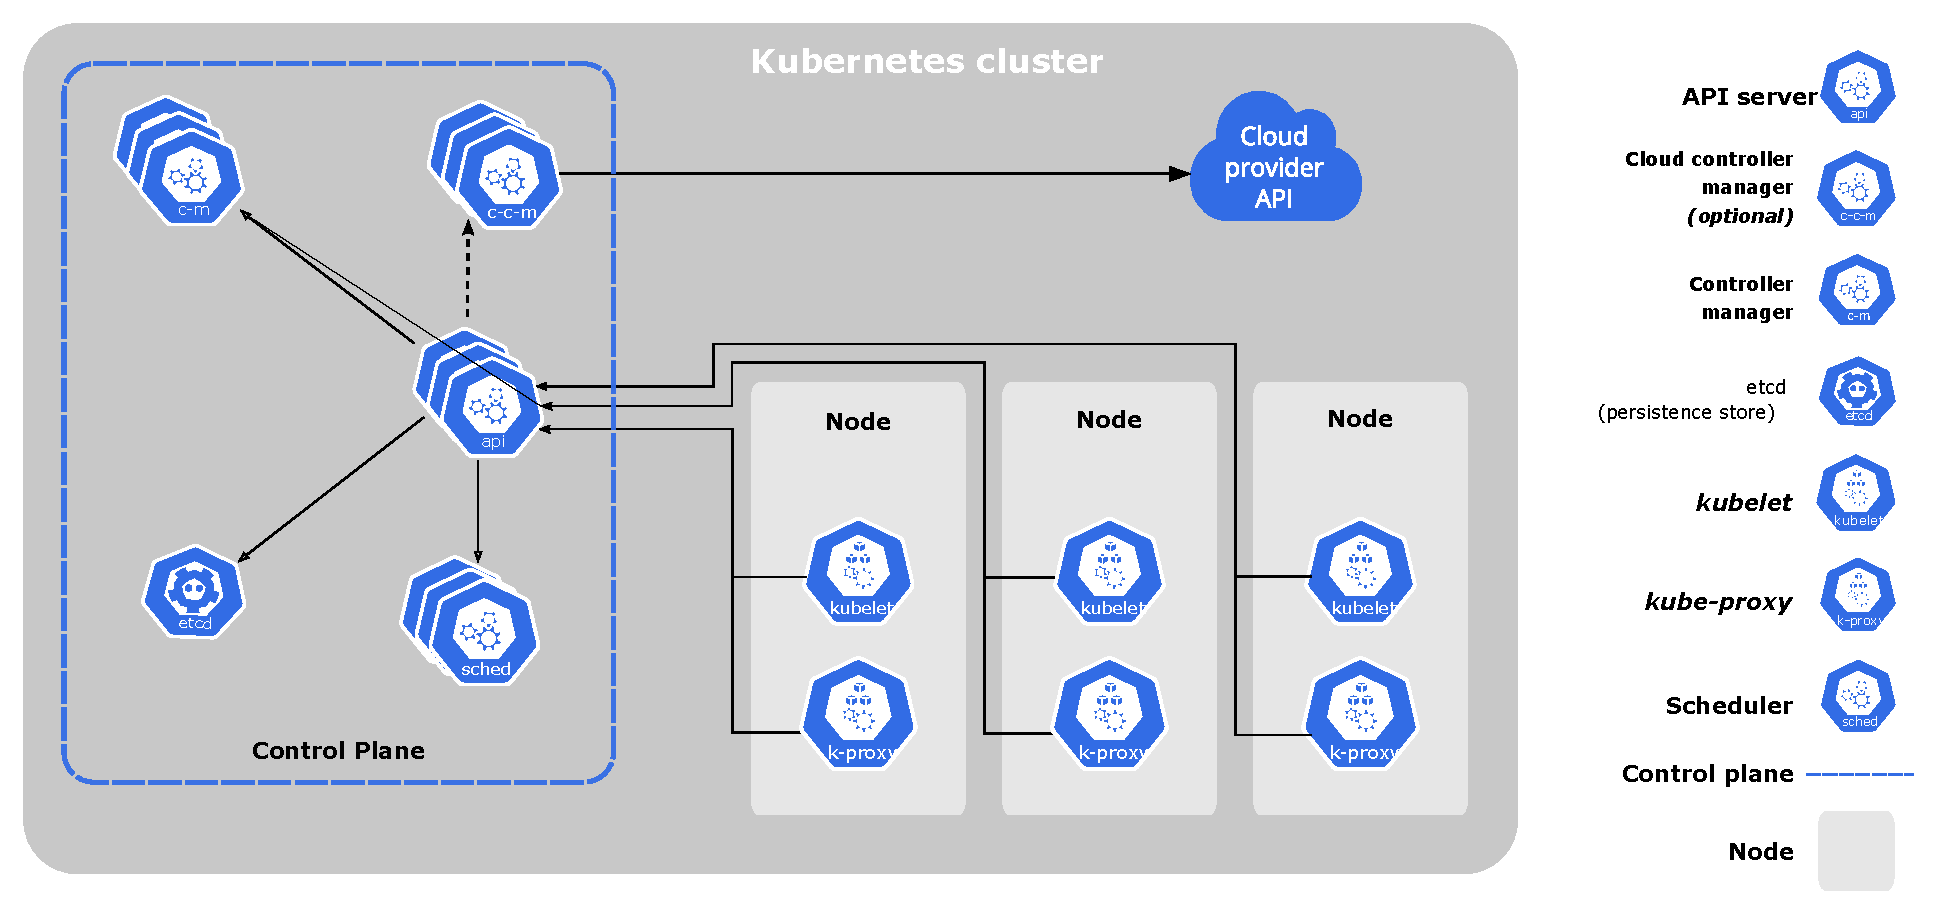
\includegraphics[width=\textwidth]{images/components-of-kubernetes.pdf}
    \caption{The components of a Kubernetes cluster~\cite{kubernetes-components}}
    \label{kube-components}
\end{figure}

A Kubernetes cluster consists of a control plane and one or more worker Nodes.
Components in the control plane manage the overall state of the cluster, while
each Node in the cluster contains a \verb|kubelet| which manages Pods and
ensures they and their containers are running via a container runtime.
Kubernetes objects are persistent entities in the Kubernetes system. They act as
``records of intent" and describe the cluster's desired state: once created, the
Kubernetes system will constantly work to ensure that the objects exists. The
\verb|kube-apiserver| exposes the Kubernetes HTTP API, which is used to create,
modify or delete these Kubernetes objects.

\subsection{Scheduling in Kubernetes}
In Kubernetes, Pods are the smallest deployable units of computing that you can
create and manage. It represents a single instance of a running
process in your cluster and typically contains one or more containers that are
tightly coupled and share resources. While Pods can be individually created,
the Kubernetes API also provides workload objects to manage multiple pods:
objects that represent a higher abstraction level than a Pod, and the Kubernetes
control plane uses the workload's specification to manage Pod objects on your
behalf. This dissertation will use the following:
\begin{itemize}
    \item \textbf{Deployment:} manages a set of Pods to run an application
        workload and typically doesn't maintain state~\cite{}.
    \item \textbf{DaemonSet:} ensures that all (or some) Nodes run a copy of a
        Pod to provide Node-local facilities~\cite{}.
    \item \textbf{Job:} creates one or more Pods and will continue to retry
        execution of the Pods until a specified number of them successfully
        terminate~\cite{}.
\end{itemize}

Almost every Kubernetes object includes two fields: \verb|spec| and
\verb|status|. \verb|spec| is used on creation as a description of the Objects
desired state. A Pod's \texttt{spec} can define affinities and QoS classes to
influence scheduling decisions. Containers also contain a \verb|spec| field
which specifies \verb|request| and \verb|limits|. The \texttt{request} field
behaves as a set of minimum requirements and is used when scheduling Pods. In
contrast, the \texttt{limits} field is used by kernel of the Node to throttle a
container's resource usage. In Kuberentes, the resource units for
\texttt{resource} and \texttt{limits} are the following:
\begin{itemize}
    \item \textbf{CPU:} The metric used is \textit{cpu} units, where 1 cpu unit
        is equivalent to a 1 physical/virtual core. Fractional requests are
        permitted with the notation $x$m; $100$m can be read as ``one hundred
        millicpu".
    \item \textbf{Memory:} This is measured in bytes. Kubernetes also allows the
        use of quantity suffixes, such as, k, M, G, Ki, Mi, Gi.
\end{itemize}
\texttt{status} describes the current state of the object, supplied and updated
by the Kubernetes system. These fields are core to scheduling in Kubernetes.

When a Pod is created, it initially exists in a ``Pending" state: it has been
declared but hasn't yet been allocated to a Node. Kubernetes schedulers watch for
newly created but unassigned Pods, and based on a set of
rules or algorithms, select the most suitable Node for that Pod. Once a Node is
chosen, the scheduler ``binds" the Pod to the Node, updating the Pod's definition
in the Kubernetes API server by setting its \verb|spec.nodeName| field to the
name of the Node. Once this occurs, the Pod transitions from ``Pending" to
``Running".

\section{\protect\textsc{Pronto}}
This section first explains theory behind \textsc{Pronto}, which will also be
eventually used by \textsc{Carico}. We outline the motivation for this
dissertation, highlighting \textsc{Pronto}'s strengths and potential
benefits to Kubernetes scheduling. Finally, we investigate its assumptions and
empirical evidence to reveal \textsc{Pronto}'s limitations and outline
requirements of a new algorithm that produces and uses a \textbf{comparable} and
\textbf{reservable} signal to inform scheduling decisions.

\subsection{Singular Value Decomposition}
The SVD of a real matrix $\mathbf{A}$ with $m$ rows and $n$ columns where $m
\geq n$ is defines as $\mathbf{A} = \mathbf{U}\Sigma\mathbf{V}^T$. Here, $\mathbf{U}$ and
$\mathbf{V}$ are orthogonal matrices of shape $m \times m$ and $n \times n$
containing the left and right singular vectors, respectively. $\Sigma$ is a
rectangular matrix of shape $m \times n$ with singular values $\sigma_i$ along
its diagonal~\cite{Strang2009}.
\begin{align}
\mathbf{A} = \begin{bmatrix} a_{11} & \dots & a_{1n} \\ \vdots & \ddots & \vdots
    \\ a_{m1} & \dots & a_{mn} \end{bmatrix} = \begin{bmatrix} \mid & & \mid \\ u_1 & \ldots & u_m
\\ \mid & & \mid  \end{bmatrix} \begin{bmatrix} \sigma_1 & &  & \mid & & \mid \\ &
\ddots & & 0 & \ldots & 0 \\ & & \sigma_m & \mid & & \mid  \end{bmatrix} \begin{bmatrix}
    \text{---} & v_1^T & \text{---} \\ & \vdots & \\ \text{---} & v_m^T & \text{---} \\
    \text{---} & v_{m+1}^T & \text{---} \\ & \vdots  & \\ \text{---} & v_n^T & \text{---}
\end{bmatrix}
\end{align}

SVD can also be written compactly by discarding the elements which do not
contribute to $\mathbf{A}$.
\begin{align}
\mathbf{A} = \begin{bmatrix} \mid & & \mid \\ u_1 & \ldots & u_m
\\ \mid & & \mid  \end{bmatrix} \begin{bmatrix} \sigma_1 &
        & \\ & \ddots & \\ & & \sigma_m \end{bmatrix} \begin{bmatrix} \text{---}
& v_1^T & \text{---} \\ & \vdots & \\ \text{---} & v_m^T & \text{---}
\end{bmatrix}
\end{align}

There always exists the SVD for a real matrix, but the decomposition is not
unique: if $\mathbf{A} = \mathbf{U}_1\Sigma\mathbf{V}_1^T =
\mathbf{U}_2\Sigma\mathbf{V}_2^T$ then $\Sigma_1 = \Sigma_2$ but $\mathbf{U}_1 =
\mathbf{U}_2\mathbf{B}_a$ and $\mathbf{V}_1 = \mathbf{V}_2\mathbf{B}_b$ for some
block diagonal unitary matrices $\mathbf{B}_a,
\mathbf{B}_b$~\cite{eftekhari2019moses, Strang2009}. Each column in
$\mathbf{U}$ and $\mathbf{V}$ is an eigenvector of $\mathbf{AA}^T$ and
$\mathbf{A}^T\mathbf{A}$.

\subsection{Principal Component Analysis}
Principal Component Analysis~\cite{} is a staple of linear
dimensionality-reduction techniques. The standard PCA procedure takes as input a
matrix $\mathbf{B}$ representing $n$ columns of data with $m$ dimensions and
mean-centers it: $\mathbf{A}_{ij} = (\mathbf{B}_{ij} - \mu_i)$ where $\mu_i$ is
the mean of the row $i$. The output of PCA is a set of vectors that explain most
of the variance within $\mathbf{B}$. Given the covariance of the mean-centered
matrix $\mathbf{A}$ is defined as $\mathbf{AA}^T$, the Principal Components
(PCs) maximise the following equation:
\begin{align}
\text{Var}_i = \max_{\substack{x_i \in \mathbb{R}^m \setminus \{\mathbf{0}\} \\
    \|x_i\|=1 \\ x_i \perp x_1 \dots x_{i-1}}} x_i^T \mathbf{A} \mathbf{A}^T x_i
\end{align}

As $\mathbf{A} = \mathbf{U}\Sigma\mathbf{V}^T$ from SVD,
$\mathbf{AA}^T = \mathbf{U}\Sigma\mathbf{V}^T\mathbf{V}\Sigma\mathbf{U}^T =
\mathbf{U}\Sigma^2\mathbf{U}^T$. Therefore, it can be shown that the PCs
$x_i = u_i$ from $\mathbf{U}$. The pair $\mathbf{U}, \Sigma$ will also be
referred to as a subspace as they provide sufficient information to describe the
original $\mathbf{B}$ matrix.

\subsection{Subspace-Merge}
Subspace-Merge is used to merge two subspaces together. Given two subspaces
$(\mathbf{U}_1, \Sigma_1)$ and $(\mathbf{U}_2, \Sigma_2)$ from $\mathbf{Y}_1$ and
$\mathbf{Y}_2$ respectively, the subspace of $\mathbf{Y} = [\mathbf{Y}_1,
\mathbf{Y}_2]$ is:
\begin{align}
    \mathbf{U}\Sigma = \text{SVD}([\mathbf{U}_1\Sigma_1, \mathbf{U}_2\Sigma_2])
\end{align}
$[\mathbf{A}, \mathbf{B}]$ signifies the concatenation of two matrices with the
same number of rows. This procedure doesn't use the right singular vectors,
reducing the required computations and memory.

\subsection{Incremental-SVD}
Incremental-SVD allows \textsc{Pronto} to become a streaming algorithm with limited
memory. It takes a stream of chunks $\mathbf{Y}_i$, such that  $[\mathbf{Y}_1,
\ldots, \mathbf{Y}_l] = \mathbf{Y}$, and with each recieved chunk it performs
Subspace-Merge to produce $\mathbf{U}_l, \Sigma_l$ where $\mathbf{Y} =
\mathbf{U}_l\Sigma_l\mathbf{V}_l^T$

\begin{algorithm}
\caption{Incremental-SVD}
\textbf{Data:} $\mathbf{Y} = [\mathbf{Y}_1, \dots, \mathbf{Y}_l]$ \\
    \textbf{Result:} $\mathbf{U}_l, \Sigma_l$ such that $\mathbf{Y} =
    \mathbf{U}\Sigma\mathbf{V}^T$
\begin{algorithmic}
\State $\mathbf{U}_1, \Sigma_1, \mathbf{V}_1^T = \text{SVD}(\mathbf{Y}_1)$
\For {$i = 2$ to $l$}
\State $\mathbf{U}_i, \Sigma_i, \mathbf{V}_i^T = \text{SVD}([\mathbf{U}_{i-1}\Sigma_{i-1}, \mathbf{Y}_i])$
\EndFor
\end{algorithmic}
\end{algorithm}
If the shape of the batches of data is $m \times b$, the space complexity of
Incremental-SVD is $\mathcal{O}(m^2 + mb)$ as only the latest version of
$\mathbf{U}_i,\Sigma_i$ and $\mathbf{Y}_i$ are needed for each iteration.

\subsection{FPCA and FSVD}
FPCA combines the relationship between standard SVD and PCA with the
Subspace-Merge operation, to calculate the PCs of the data $[\mathbf{Y}_1,
\ldots,\mathbf{Y}_m]$ from $m$ nodes. Every node $i$ performs perform SVD  on
their local data, to produce the subspace $\mathbf{U}_i, \Sigma_i$. These
subspaces can be merged using at most $m-1$ Subspace-Merges to obtain the global
subspace $\mathbf{U}'\Sigma'$, corresponding to the PCs of the aggregated data
from all the nodes. \textsc{Pronto} turns this procedure into a streaming algorithm, by
running Subspace-Merge on the subspaces produced by incremental-SVD. Finally,
\textsc{Pronto} also introduces a forgetting factor $\gamma$ in front of
$\mathbf{U}_i\Sigma_i$ in Incremental-SVD that allows it to ``forget" old data
by gradually reducing the influence of previous subspaces. Like with standard
PCA, FPCA can be considered as FSVD on mean-centered data.

\subsection{Low-Rank Approximations}
It can be shown that using the first $r$ eignenvectors in the above algorithms
approximate the result of using all $m$ eignenvectors, i.e. if
\begin{align}
\mathbf{Y} = \begin{bmatrix} \mid & & \mid \\ u_1 & \ldots & u_m
    \\ \mid & & \mid  \end{bmatrix} \begin{bmatrix} \sigma_1 &
        & \\ & \ddots & \\ & & \sigma_m \end{bmatrix} \begin{bmatrix} \text{---}
& v_1^T & \text{---} \\ & \vdots & \\ \text{---} & v_m^T & \text{---}
\end{bmatrix}
\end{align}
We can use $\mathbf{U}^r = \begin{bmatrix} \mid & & \mid \\ u_1 & \ldots & u_r
    \\ \mid & & \mid  \end{bmatrix}$ and $\mathbf{\Sigma}^r = \begin{bmatrix}
\sigma_1 & & \\ & \ddots & \\ & & \sigma_r \end{bmatrix}$ where $r \leq m$ in
Incremental-SVD and Subspace-Merge. This lets \textsc{Pronto} reduce the number of
computations it performs and its memory usage.

\subsection{\protect\textsc{Pronto} System Overview}
\begin{figure}[ht]
    \centering
    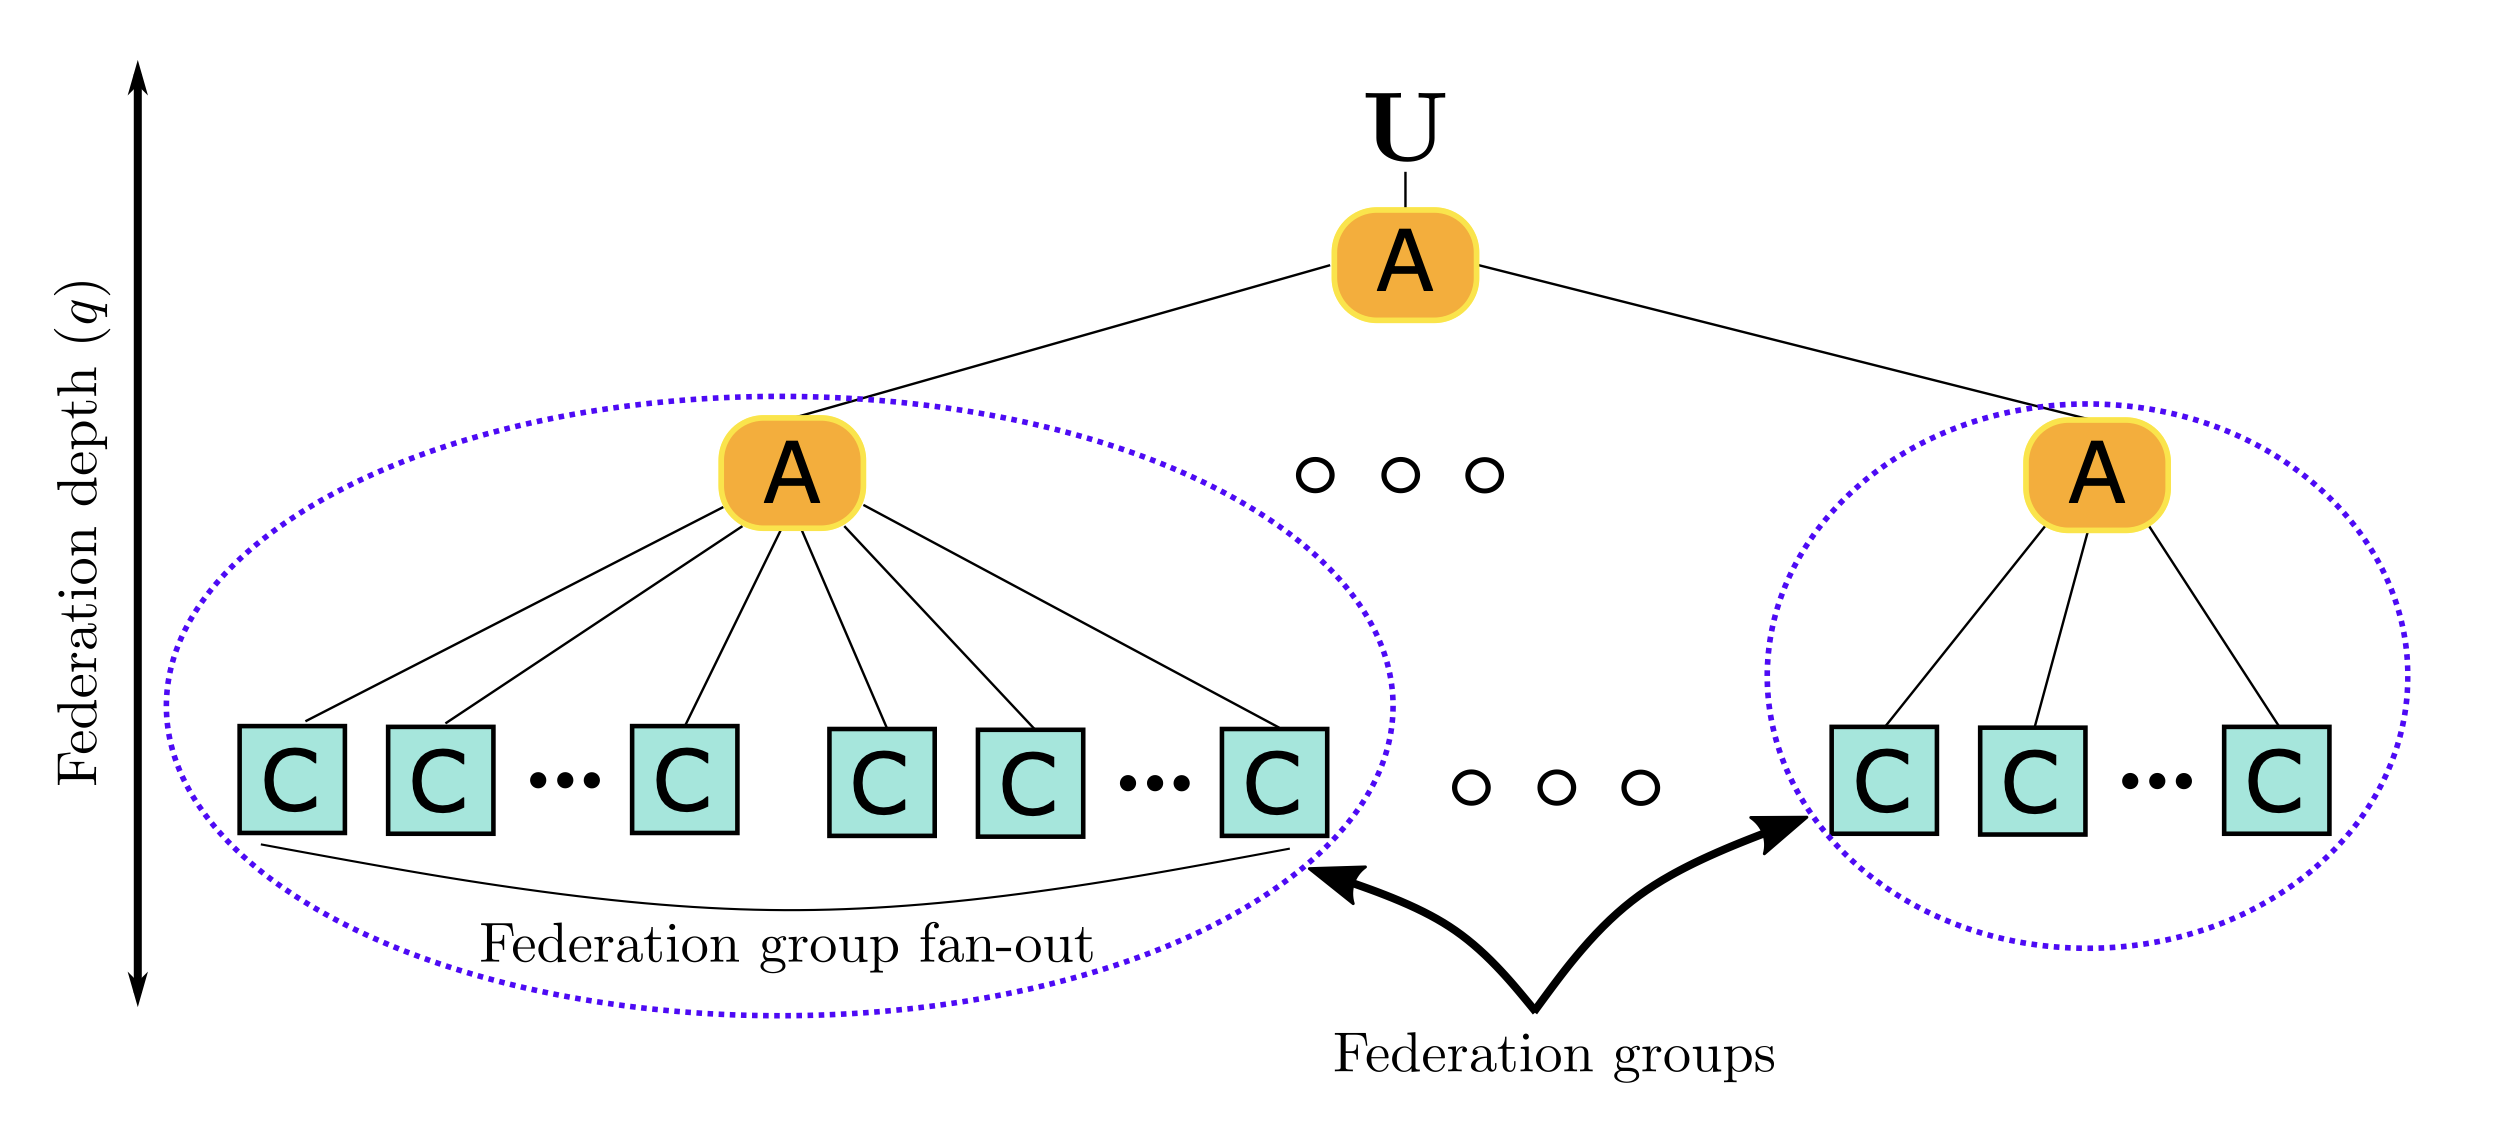
\includegraphics[width=\textwidth]{images/pronto-agg.png}
    \caption{How local models are aggregated in \textsc{Pronto}. Dedicated aggregator
    nodes propagate the updated subspaces until the root is reached~\cite{grammenos_pronto_2021}.}
    \label{pronto-agg}
\end{figure}
There are two types of nodes in \textsc{Pronto} (Figure \ref{pronto-agg}):
compute node (C) and aggregator node (A). Compute nodes collect and center
telemetry (i.e. CPU and Memory) and perform Incremental-SVD to obtain the low
rank approximations of the local subspace $\mathbf{U},\Sigma$. The aggregator
nodes perform Subspace-Merge on incoming subspaces, with subspace produced by
the root aggregator node being propagated back to the compute nodes.

\subsection{\protect\textsc{Pronto} Reject-Job Signal}
\begin{figure}[ht]
    \centering
    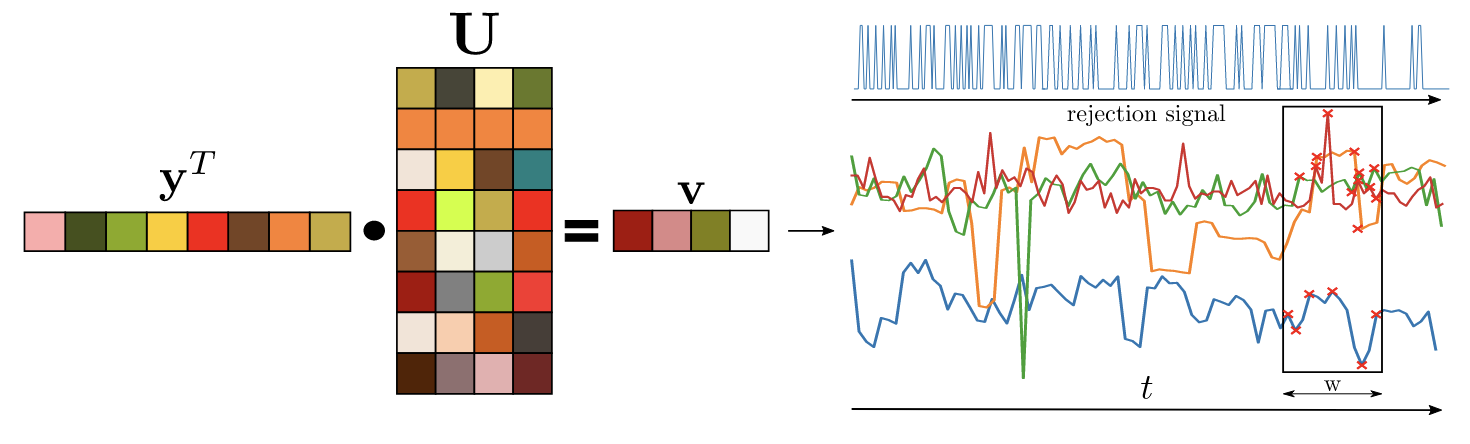
\includegraphics[width=\textwidth]{images/pronto}
    \caption{Projection of incoming $y \in \mathbb{R}^d$ onto embedding $U \in
    \mathbb{R}^{d \times r}$ producing $R$ projections in $v \in \mathbb{R}^{1
    \times r}$. Projections are tracked over time for detecting spikes which
    form the basis of the rejection signal. The sliding window for spike
    detection for each projection is of size $w$ also shown in the figure.}
    \label{pronto-components}
\end{figure}

\textsc{Pronto} performs peak detection to estimate performance degradation
(Figure \ref{pronto-components}) Each compute node projects their data onto the
latest version of $\textbf{U}$, and identifies all the spikes. If the weighted
sum of these spikes, using the corresponding singular values in $\Sigma$,
exceeds a threshold, a ``Reject-Job" signal is raised to indicate that the node
is potentially experiencing performance degradation and a task should not be
scheduled on that node.

\subsection{Strengths}
\textsc{Pronto}'s core strength is its ability to leverage global telemetry data
to predict performance degradation with high accuracy. The orginal
\textsc{Pronto} paper~\cite{grammenos_pronto_2021}, which compared its
effectiveness against non-distributed dimensionality-reduction methods,
demonstrated superior performance in predicting CPU-Ready spikes in real-world
datacenter traces. This improved accuracy over the non-distributed
strategies suggests that a federated approach allows for a more comprehensive
understanding of system-wide resource contention, providing more accurate
contention predictions than with only individual node data. These compelling
results indicate a strong potential benefit from applying \textsc{Pronto}
underlying principles to Kubernetes where efficient resource management is
paramount.

\subsection{Weaknesses}
\label{sec:intro-weakness}
While \textsc{Pronto} offers a promising approach to performance prediction, its
direct application within a Kubernetes environment faces significant challenges
due to fundamental communication assumptions and practical limitations of
peak-prediction.

\subsubsection{Assumptions}
Implementing \textsc{Pronto} in a complex system like Kubernetes raises
fundamental challenges:
\begin{enumerate}
    \item \textbf{Zero-Latency Assumption:} A critical assumption in the
        \textsc{Pronto} paper is the absence of communication latency, and
        implicitly binding latency. This implies that scheduled workloads are
        immediately reflected in a node's telemetry, and therefore, its
        Reject-Job signal. In such a scenario, a central scheduler could
        instantaneously stop assigning workloads once a Node signal potential
        degredation. However, this assumption does not hold in real-world
        Kubernetes clusters. The latency between a pod being bound to a Node and
        that Pod actually starting to run and consume resources has been shown
        to reach as high as 4 seconds \cite{qadeer_scaling_2022}. Directly
        applying \textsc{Pronto}'s binary signal in this high-latency
        environment could lead to a ``runaway train" schenario": Nodes might
        advertise willingness to accept new Pods while a large number of
        ``inflight" Pods are still pending startup and will overload the node
        once active. This highlights the need for a reservation mechanism for
        a node's signal.
    \item \textbf{Lack of Explicit Allocation Algorithm:} \textsc{Pronto} allows
        individual compute nodes to reject or accept incoming jobs. However, it
        does not explicitly provide a system to optimally decide which compute
        nodes are considered for a task. While a simple approach would be to allow
        individual Nodes to request Pending Pods, it will struggle to scale.
        Having hundreds of Nodes sending requests to \texttt{kube-apiserver}
        would greatly degrade its performance or even cause it to crash.
        Instead, I decided to take a centralised approach, where Nodes
        periodically send their signal to a central scheduler to influence where
        Pods are allocated.
    \item \textbf{Limited Scoring Capability:} Unlike typical Kubernetes
        schedulers that employ a scoring-function to rank Nodes and select the
        ``optimal" fit~\cite{kube-scheduler}, a binary signal offers no
        mechanism to differentiate between suitable Nodes. This could lead to
        suboptimal allocation decisions, potentially reducing overall cluster
        throughput and efficiency. Thus, Nodes would need to produce a
        comparable signal.
\end{enumerate}

% The Pronto paper implements a binary "responsiveness" signal which predicts
% upcoming performance degradation. Because the authors assume a system with no
% communication latency (implicitly assuming that scheduled workloads were
% immediately visisble in the signal as well), they could send this signal
% directly to a central scheduler which could then stop assigning workloads once a
% node sent a Reject Signal.
%
% However, due to significant pod startup latency, the method can't be used in a
% real-world Kubernetes cluster is infeasible. When measuring pod startup in a
% 100 node clusters, the more than 50\% of pods took more than $\approx$ 1 second
% to startup. In addition, when nodes were 100\% full, pod startup could reach up
% to 4 seconds. This latency is significant when Kubernetes schedulers can
% support a throughput of $\approx$1000 pods per second
% \cite{qadeer_scaling_2022}. Applying the same approach as used in the paper,
% could result in nodes advertising a "willingness" to take on new pods while
% a large number of pods are in "flight" and once running will immediately
% overload the node. To prevent this runaway train type problem, I need to define
% a reservation function: a function that reserves an amount of the signal for a
% bound pod. This is necessary to allow previous scheduling decisions to have an
% imnpact on the signal while the signal updates to take into account the
% scheduled pods.
%
% In addition, telemetry-based schedulers can use individual node performance
% information to score and fine-tune pod allocations. A binary signal does not
% provide the necessary information for scoring nodes, potentially resulting in
% worse pod allocations.
%
% In summary, the requirements of the signal are:
% \begin{itemize}
    % \item Reservable: the scheduler must be able to track the pending impact of
        % previous scheduling decisions until the pods have begun running.
    % \item Comparable: the signal must provide enough information to score nodes
% \end{itemize}

\subsubsection{Peak-Prediction}
\textsc{Pronto} uses peak-prediction on collected telemetry to predict future
performance degradation. For \textsc{Pronto} to generate an accurate Reject-Job
signal in Kubernetes, the chosen contention metrics should exhibit clear,
distinguishable spikes during genuine high-resource contention. While increasing
the number of collected metrics can help reduce the impact of erroneous spikes,
collecting more telemetry and operating on larger matrices will incur additional
overheads and reduce the available resources for Pods.

\textsc{Pronto} used metrics, like CPU-Ready, specific to virtual machines
(VMs), limiting its application to Kubernetes clusters with only VMs.
Linux-based systems offer alternative Pressure Stall Information (PSI)
metrics, accessible via \texttt{/proc/pressure/<cpu|memory|io>}. These
pseudo-files track the time tasks are stalled waiting for resources. To
investigate the feasibility of using PSI for peak prediction within a Kubernetes
Node, I polled the polled the \verb|/proc/pressure| files under different
workloads.

\begin{figure}[htbp] % Added 'b' and 'p' for better placement flexibility
    \centering % Centers the entire figure

    % --- First Row ---
    \begin{subfigure}[b]{0.48\textwidth} % [b] for bottom alignment, 0.48\textwidth for width
        \centering
        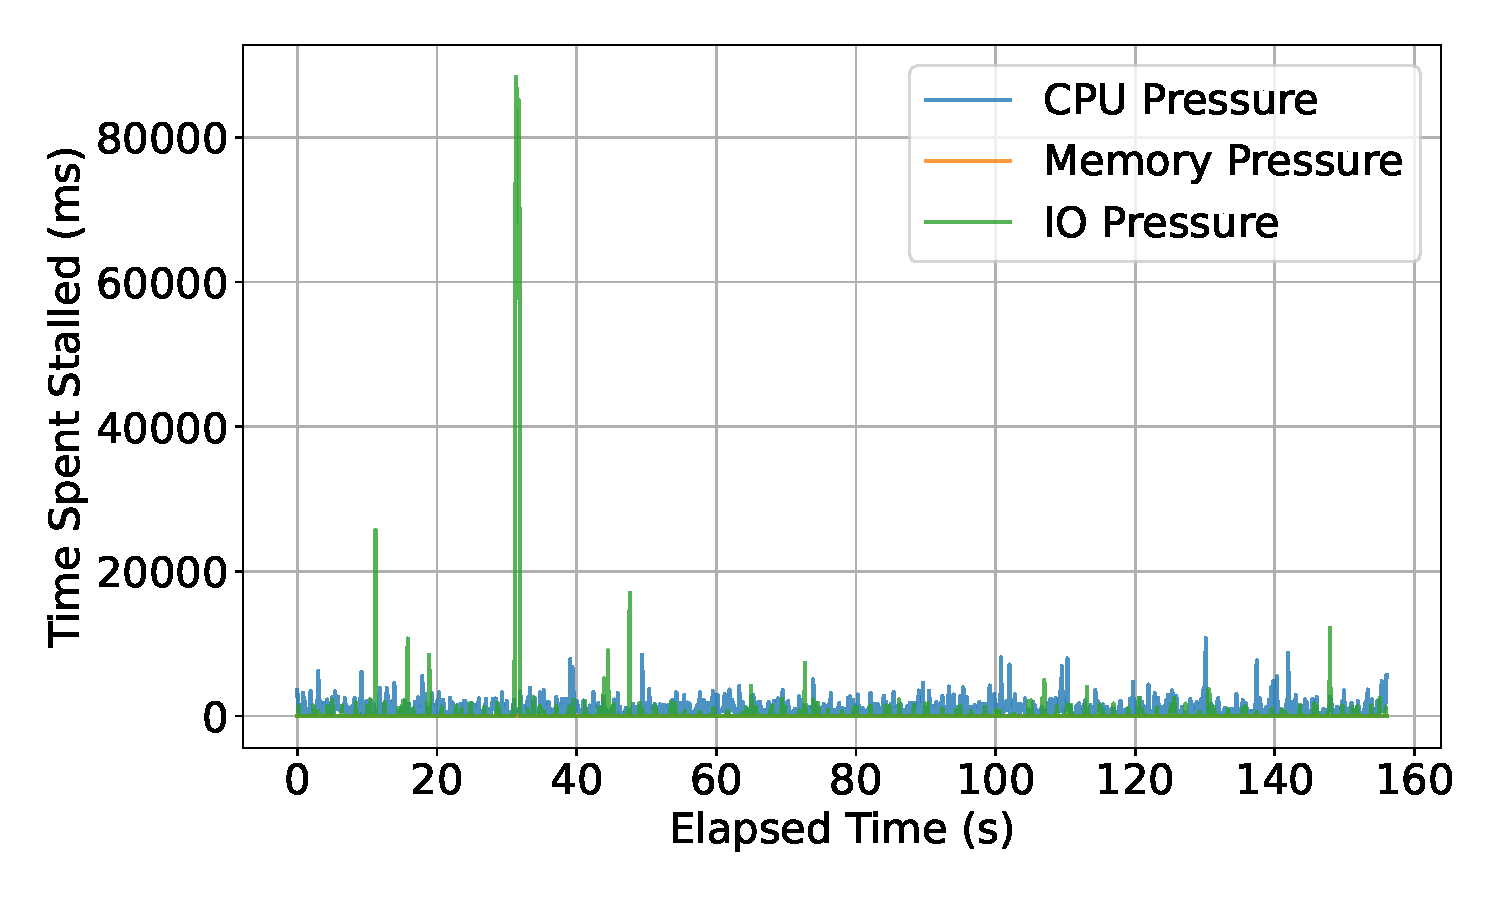
\includegraphics[width=\linewidth]{images/pressure-baseline.pdf}
        \caption{PSI when no Pods are running} % Specific caption for this graph
        \label{fig:pressure-baseline} % Individual label
    \end{subfigure}%
    \hfill % Adds horizontal space between subfigures
    \begin{subfigure}[b]{0.48\textwidth}
        \centering
        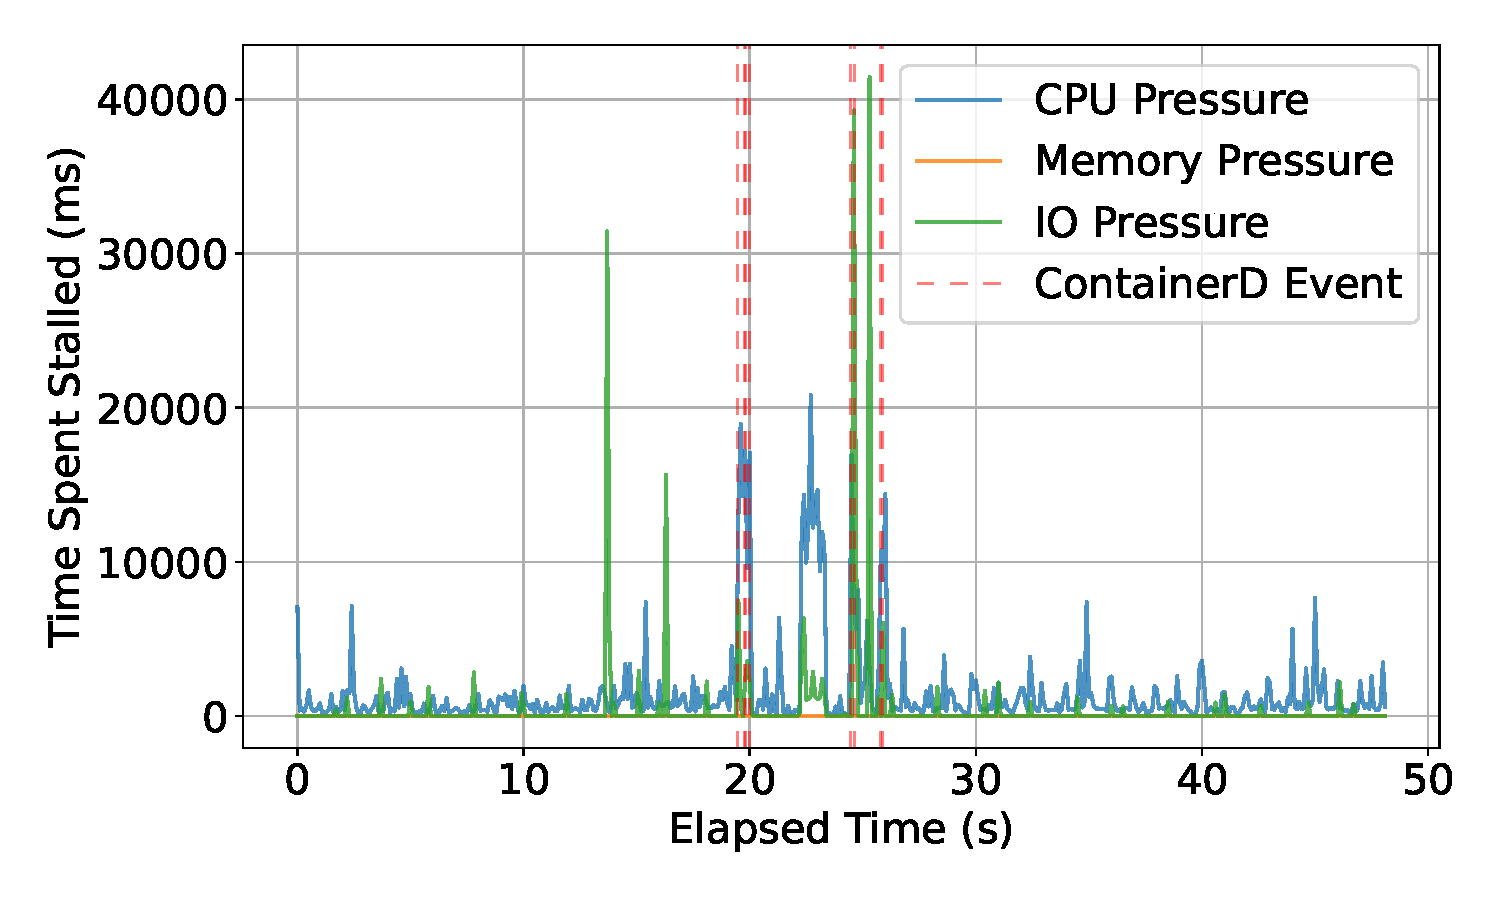
\includegraphics[width=\linewidth]{images/pressure-single.pdf}
        \caption{PSI when running a single Pod} % Specific caption for this graph
        \label{fig:pressure-single}
    \end{subfigure}
    \\[1em] % Forces a new line with 1em vertical space between rows

    % --- Second Row ---
    \begin{subfigure}[b]{0.48\textwidth}
        \centering
        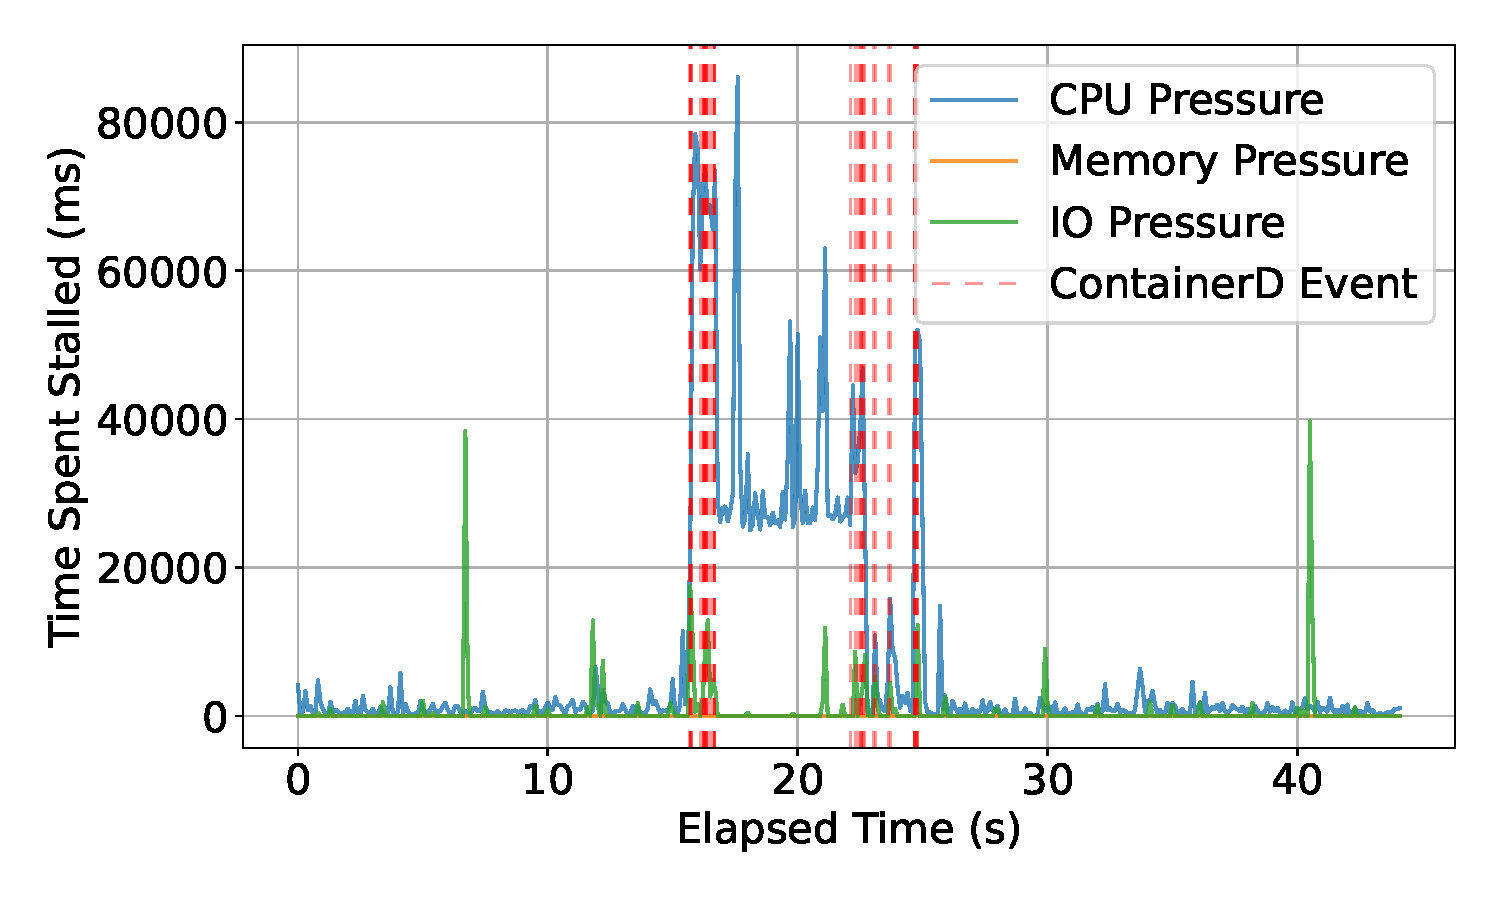
\includegraphics[width=\linewidth]{images/pressure-smallbatch.pdf}
        \caption{PSI when running 5 Pods} % Specific caption for this graph
        \label{fig:pressure-smallbatch}
    \end{subfigure}%
    \hfill
    \begin{subfigure}[b]{0.48\textwidth}
        \centering
        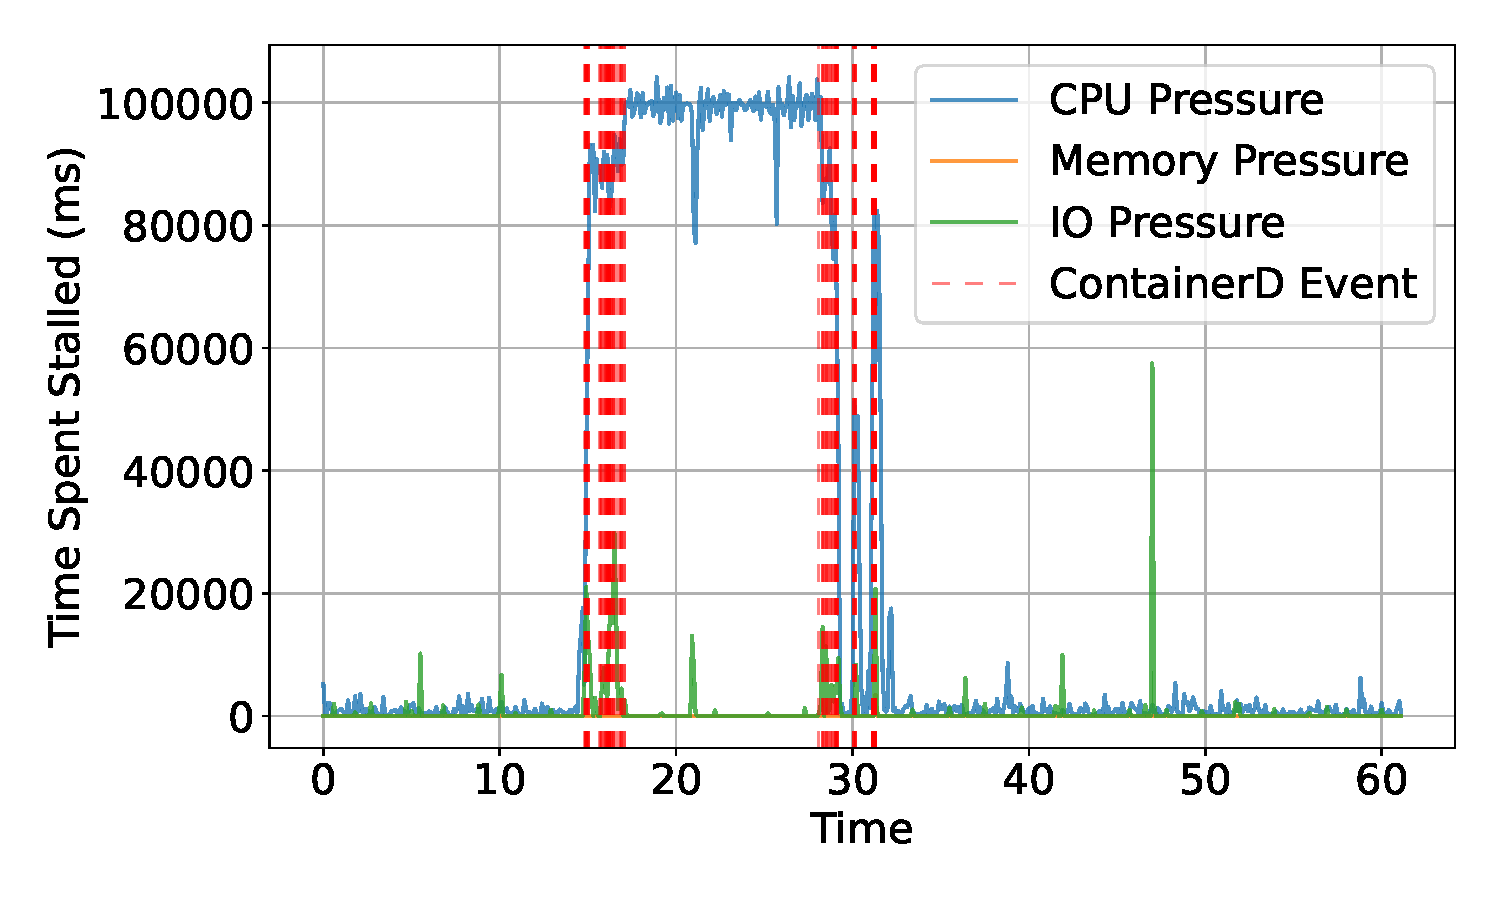
\includegraphics[width=\linewidth]{images/pressure-bigbatch.pdf}
        \caption{PSI when running 10 Pods} % Specific caption for this graph
        \label{fig:pressure-bigbatch}
    \end{subfigure}

    \caption{Measurements of \texttt{total} from \texttt{/proc/pressure/} when
    running different sized Jobs with Pods executing \texttt{bpi(2000)}. Spikes
    are observed across all workloads.} % Enhanced overall caption
    \label{fig:pressure-combined} % New label for the combined figure
\end{figure}

Figure \ref{fig:pressure-combined} shows how lightweight workloads can still cause the
PSI metrics to experience significant spikes. These transient spikes
can be attributed to the container runtime (e.g. Containerd) consuming resources
during the creation or deleteion of containers. This ``noise" would be
difficult to distinguish from genuine indicators of resource contention ,
compromising the accuracy of \textsc{Pronto}'s peak-detection mechanism.

\begin{figure}[htbp] % Added 'b' and 'p' for better placement flexibility
    \centering % Centers the entire figure

    % --- First Row ---
    \begin{subfigure}[b]{0.48\textwidth} % [b] for bottom alignment, 0.48\textwidth for width
        \centering
        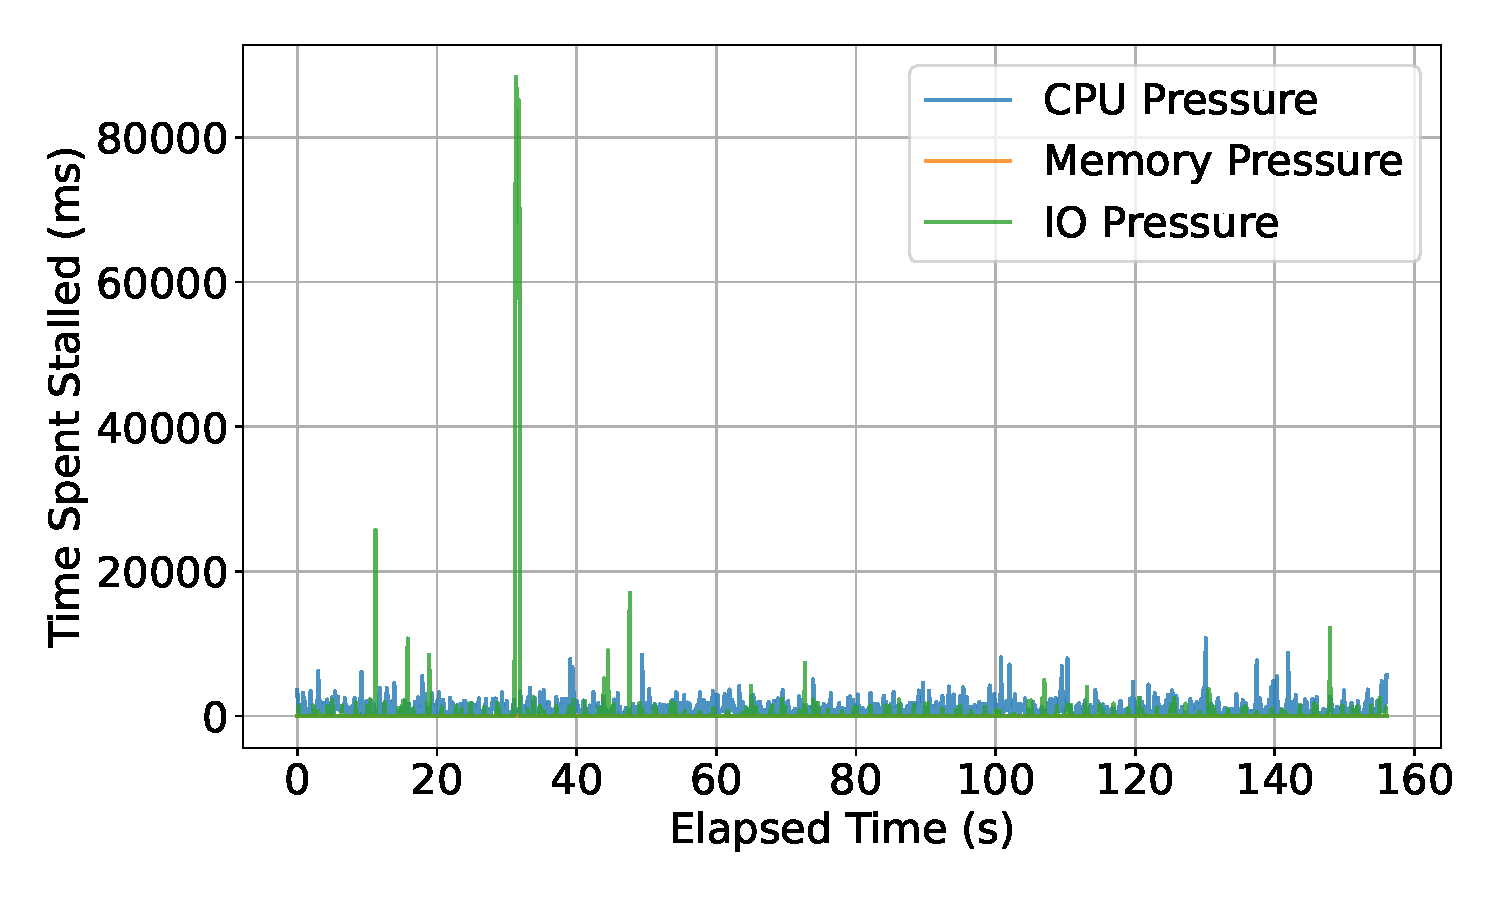
\includegraphics[width=\linewidth]{images/pressure-baseline.pdf}
        \caption{PSI when no Pods are running} % Specific caption for this graph
        \label{fig:avg-pressure-baseline} % Individual label
    \end{subfigure}%
    \hfill % Adds horizontal space between subfigures
    \begin{subfigure}[b]{0.48\textwidth}
        \centering
        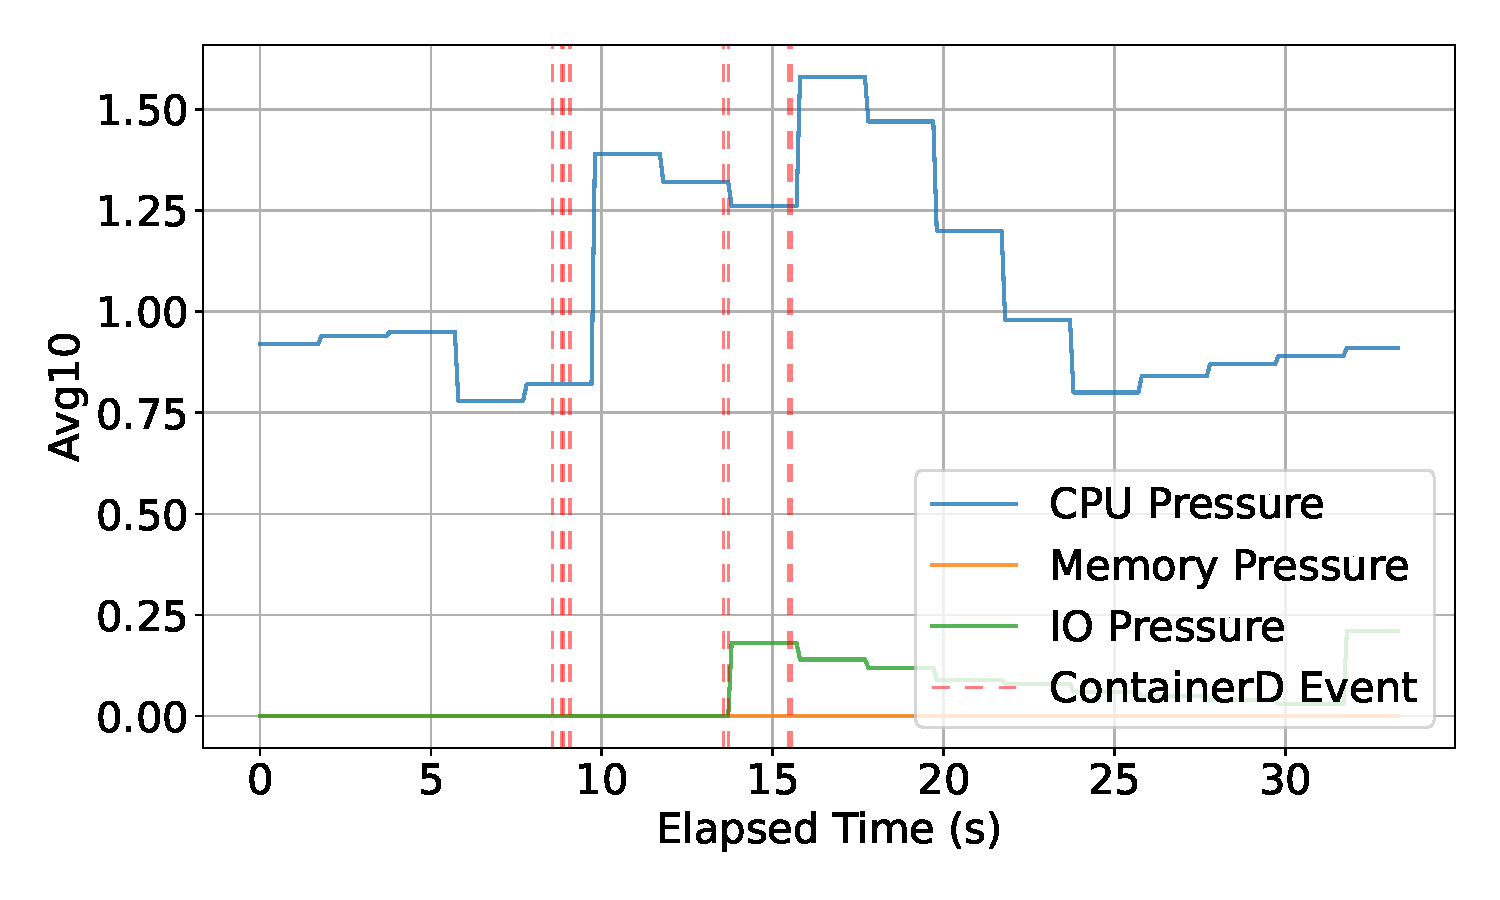
\includegraphics[width=\linewidth]{images/avg-pressure-single.pdf}
        \caption{PSI when running a single Pod} % Specific caption for this graph
        \label{fig:avg-pressure-single}
    \end{subfigure}
    \\[1em] % Forces a new line with 1em vertical space between rows

    % --- Second Row ---
    \begin{subfigure}[b]{0.48\textwidth}
        \centering
        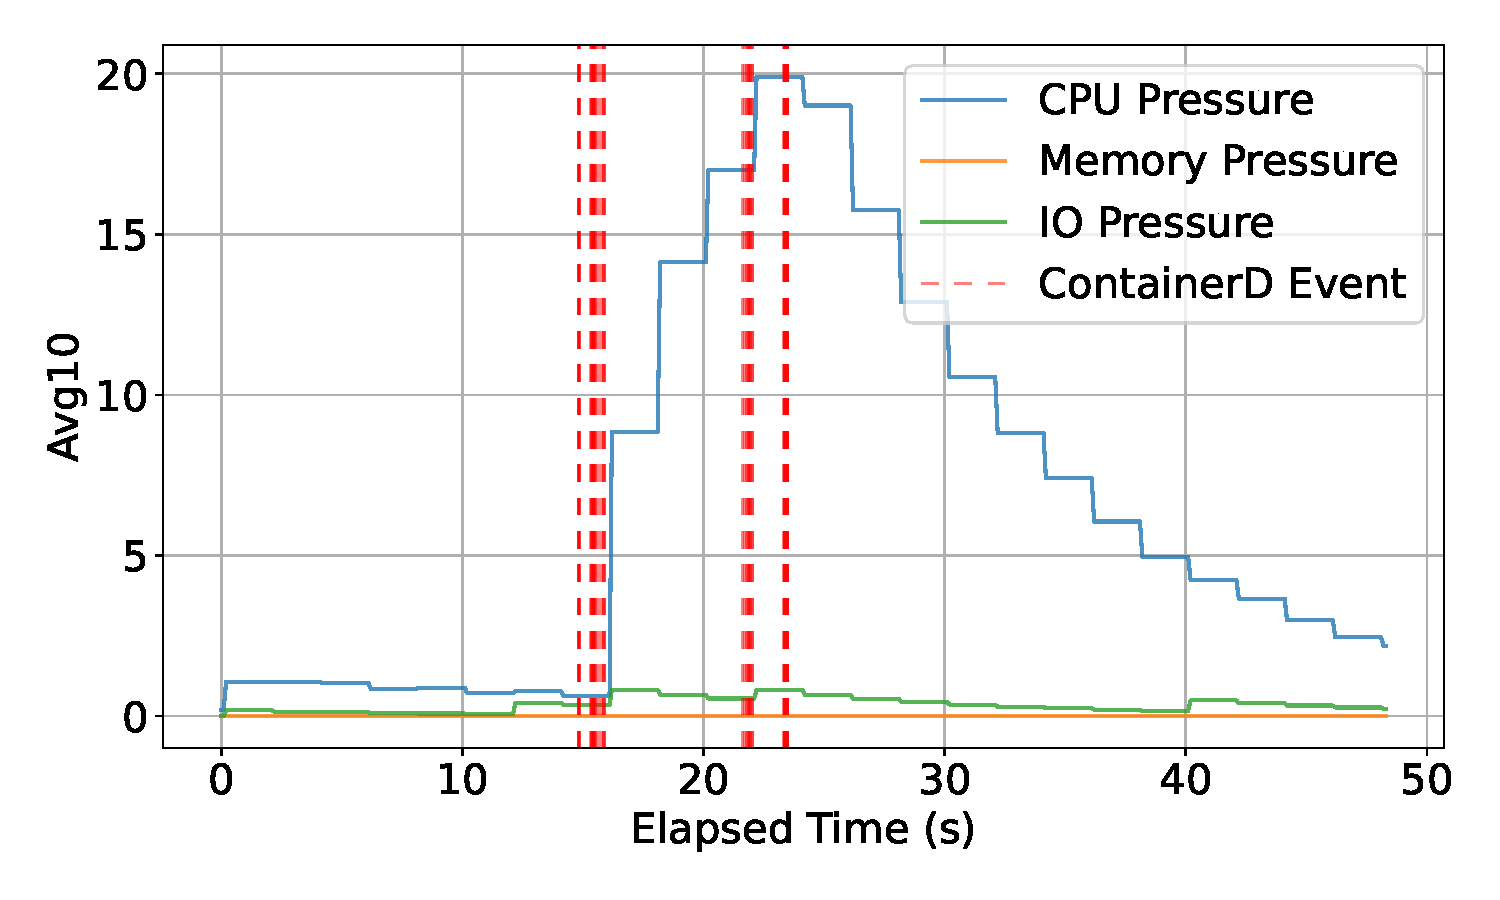
\includegraphics[width=\linewidth]{images/avg-pressure-smallbatch.pdf}
        \caption{PSI when running 5 Pods} % Specific caption for this graph
        \label{fig:avg-pressure-smallbatch}
    \end{subfigure}%
    \hfill
    \begin{subfigure}[b]{0.48\textwidth}
        \centering
        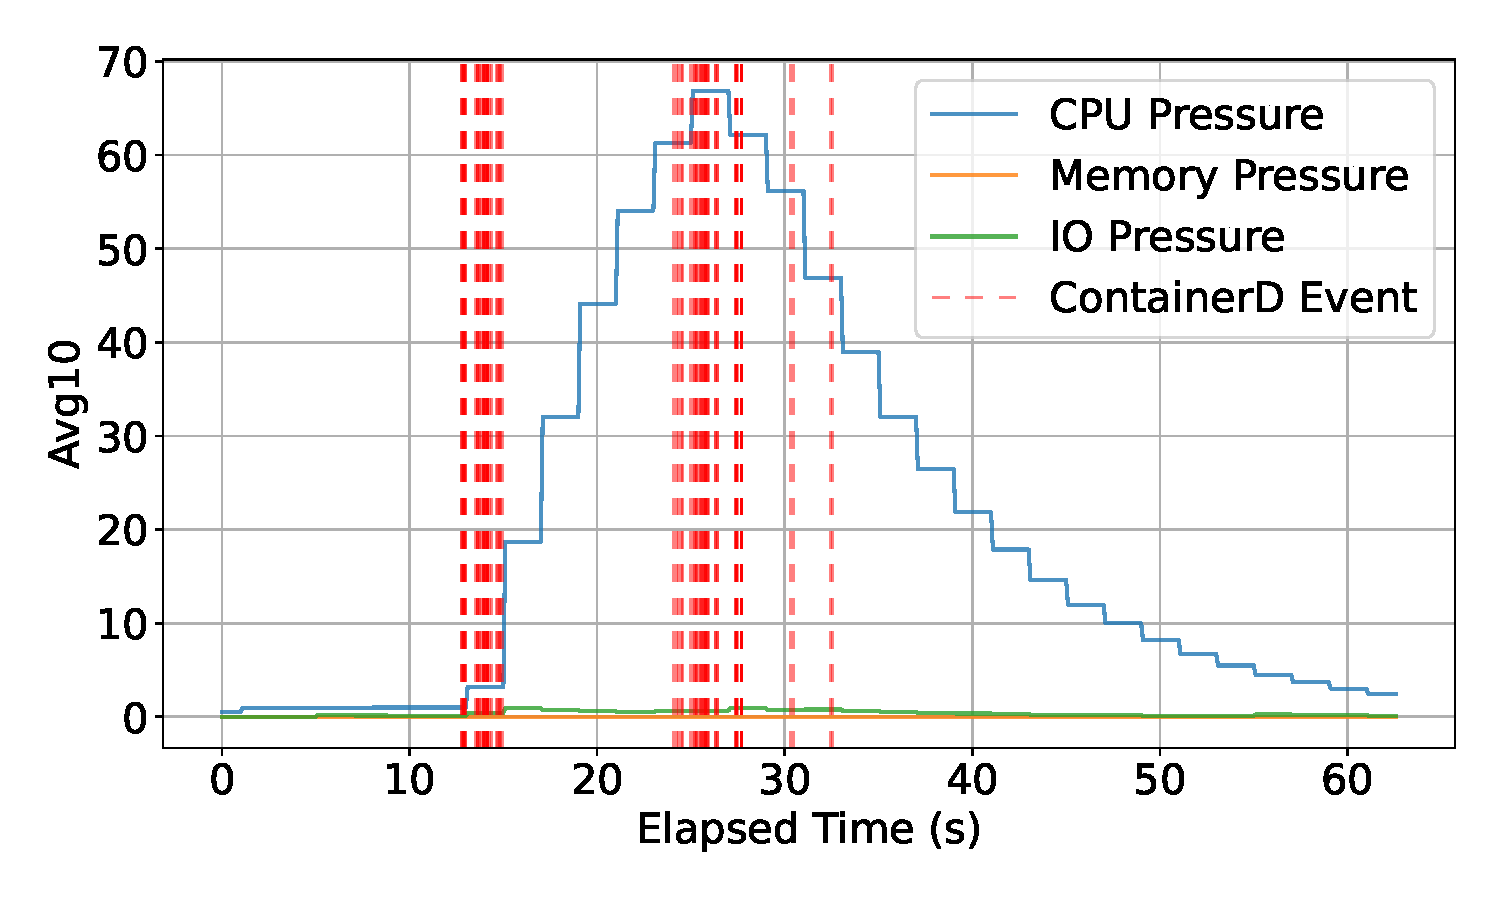
\includegraphics[width=\linewidth]{images/avg-pressure-bigbatch.pdf}
        \caption{PSI when running 10 Pods} % Specific caption for this graph
        \label{fig:avg-pressure-bigbatch}
    \end{subfigure}
    \caption{Measurements of \texttt{avg10} from \texttt{/proc/pressure/} when
    running different sized Jobs with Pods executing \texttt{bpi(2000)}. The
    average fails to respond quickly to large contention.} % Enhanced overall caption
    \label{fig:pressure-avg}
\end{figure}

The PSI metrics also expose an average over a 10-second window. Figure
\ref{fig:pressure-avg} illustrates that averaging the PSI metrics can indeed
reduce the impact of these container runtime-induced spikes. However, this
smoothing comes at the cost of responsiveness. In the experiments running 10
Pods, the averaged metrics failed to converge on the true value observed in
Figure \ref{fig:pressure} before the Pods had finished running. This delay could
still result in the same ``runaway train" situation described earlier.

Based on this early empirical investigation, I conclude that peak-prediction on
sub-second polling of raw PSI metrics is not feasible within the noisy
Kubernetes environment.

\section{Next Steps}
These weaknesses highlight the requirements for a more sophisticated federated
scheduler:
\begin{enumerate}
    \item \textbf{Comparable and Reservable Signal:} Node's will generate a
        signal that: 1) provides enough information to score and rank
        Nodes effectively, and 2) allows the scheduler to track the pending impact
        of previous scheduling decisions until Pods have begin running.
    \item \textbf{Centralised Architecture:} A central scheduler will use
        Nodes' scores to determine Pod allocation perform the ``bind" operation.
    \item \textbf{Avoids Peak Prediction:} Telemetry generated by Node is too
        noisy to perform low-dimensionality peak-prediction.
\end{enumerate}




% In the paper, Pronto uses \verb|CPU-Reeady| which is generated by the VMware
% vSphere virtualisation platform. This metric can't be used within a
% Kubernetes cluster as machines can be both virtual and physical. Since Linux
% 4.20+, the kernel can track how long tasks are stalled waiting for the CPU
% at a cgroup granularity. By inspecting the the root cgroup’s CPU pressure
% file using \verb|cat /proc/pressure/cpu| you can measure the total time all
% processes spent waiting for the CPU to be available.
%
% While this type of metric can be used to alert of performance degradation,
% this metric has a few shortcomings. Firstly, it only reports CPU-centric
% information. This is not always representative measure of resource
% contention as memory-heavy workloads may starve for RAM resources while
% metrics like \verb|CPU-Ready| and \verb|/proc/pressure/cpu| remain
% unaffected.
%
% Secondly, a significant amount of resources are used starting up or deleting
% containers. This results in large spikes, as shown in figure
% \ref{pressure-eval}, which are difficult to distinguish from genuine CPU-Ready
% spikes. As Pronto uses spike detection to predict future resource performance
% degradation, container start-ups could produce detectable spikes which would
% reduce the rate at which pods are assigned to nodes and could result in lower
% throughput.
%

\section{Summary}
This chapter provided the foundational knowledge for the dissertation,
introducing an overview of the Kubernetes architecture and its scheduling
mechnaism. It then introduced \textsc{Pronto}, a novel approach to scheduling,
explaining the core mathematics behind its FPCA, and highlighting its accuracy
in predicting performance degradation through global telemetry. Finally, we
identified significant limitations of \textsc{Pronto}, and produced the
requirements for a more sophisticated federated algorithm for Kubernetes scheduling.
% \begin{tcolorbox}[boxsep=0mm,left=2.5mm,right=2.5mm]
    % \textbf{Summary:} {\em In this chapter I will summarise the problem and
    % problem space. I will review the findings of the related work, highlighting
    % weaknesses of existing Kubernetes schedulesr with respect to QoS
    % scheduling.}
% \end{tcolorbox}

